\section{Background}\label{sec:background}

Blockchain is a relatively recent technology that can be complex to grasp. At
its core, it relies on cryptographic principles to ensure secure and
transparent transactions. In this section, we will explain key blockchain
concepts, including how wallets work and interact with the blockchain, in
Sections~\ref{subsec:interacting_with_the_blockchain}
and~\ref{subsec:blockchain}, while also exploring prominent blockchain
networks, token standards, and the rise of NFTs.
Figure~\ref{fig:blockchain_concepts} provides a visual overview of these
concepts, which will be detailed in the following subsections: Wallets
\textbf{(1)} in Section~\ref{subsec:wallets}, Networks \textbf{(2)} in
Section~\ref{subsec:networks}, and Smart Contracts \textbf{(3)} in
Section~\ref{subsec:smart_contracts}. We'll also explain more technical
concepts in the scope of this project, like Solidity \textbf{(4)} in
Section~\ref{subsec:solidity}, Token Standards \textbf{(5)} in
Section~\ref{subsec:token_standards}, and NFTs \textbf{(6)} in
Section~\ref{subsec:nfts}.

\begin{figure}[H]
    \centering
    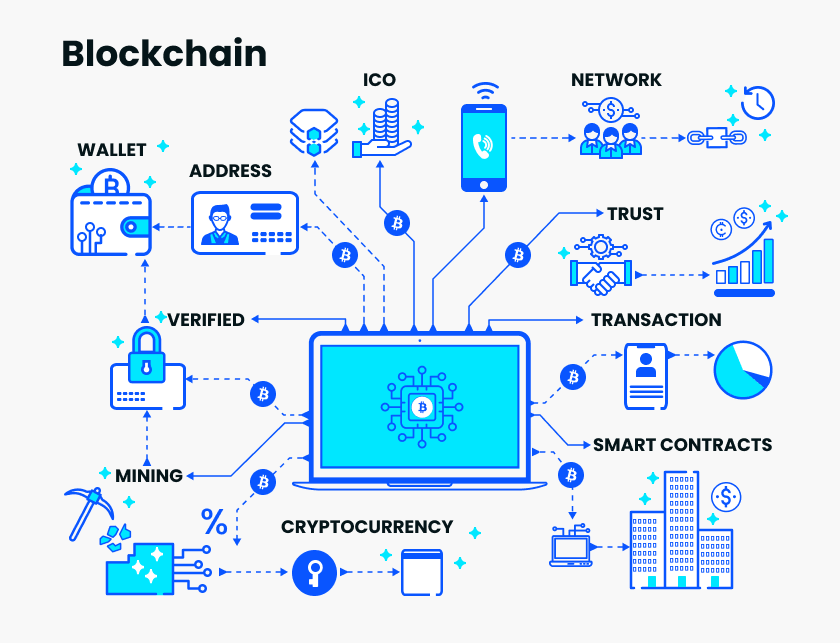
\includegraphics[width=0.5\textwidth]{Blockchain concepts.png}
    \caption[Key concepts of blockchain technology]{Key concepts of blockchain technology. Adapted from~\cite{blockchain_concepts}}\label{fig:blockchain_concepts}
\end{figure}

\subsection{Interacting with the Blockchain}\label{subsec:interacting_with_the_blockchain}

A blockchain operates as a decentralized network of nodes, each maintaining a
full copy of the blockchain. To interact with the blockchain, users send
transactions to the network, which are validated and added to blocks by nodes.
This process requires a wallet—an application that allows users to manage
digital assets, interact with smart contracts, and initiate transactions.
Wallets provide a user-friendly interface to sign transactions, manage keys,
and view account balances. Figure~\ref{fig:how_does_a_blockchain_work}
illustrates the steps involved in a blockchain transaction.

\begin{figure}[H]
    \centering
    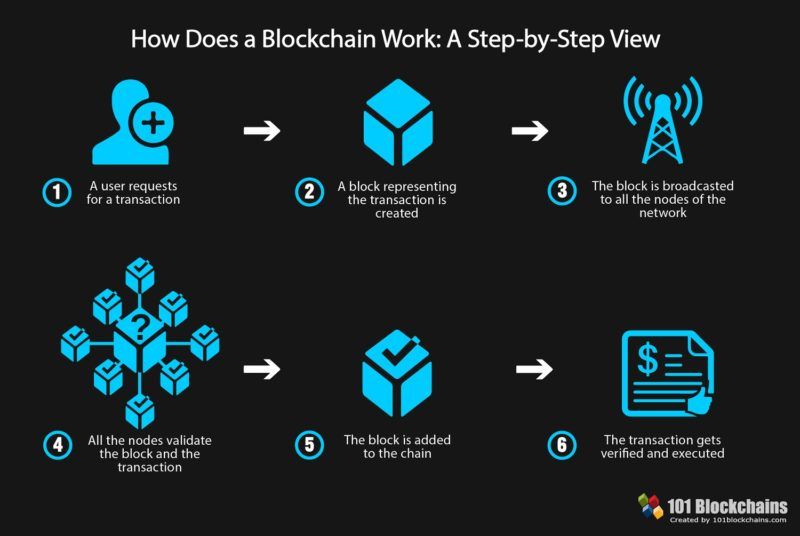
\includegraphics[width=0.66\textwidth]{How does a blockchain work.jpg}
    \caption[Blockchain transaction process]{Overview of blockchain transaction processes. Extracted from~\cite{how_blockchain_works}}\label{fig:how_does_a_blockchain_work}
\end{figure}

To execute a transaction, the user must sign it with their private key, proving
ownership of the assets being transferred (step 1). The transaction is then
broadcasted to the network (steps 2 and 3), validated by nodes (step 4), and
added to the blockchain ledger, where it becomes immutable and accessible to
all network participants (steps 5 and 6).

While transactions require signatures to alter the blockchain, reading data
from the blockchain is signature-free; users can freely query the blockchain
for information.

\subsection{Blockchain}\label{subsec:blockchain}

Blockchain is a decentralized and distributed ledger technology that enables
secure and transparent data sharing across a network. A blockchain consists of
a series of blocks, each containing a list of transactions. These blocks are
linked in chronological order, forming a tamper-proof record. Key
characteristics of blockchain technology include:

\paragraph{Decentralization:}
Blockchain operates on a decentralized network of nodes, eliminating the need
for central control and reducing points of failure.

\paragraph{Transparency:}
Data on the blockchain is visible to all participants, fostering trust and
accountability, as transactions can be verified independently.

\paragraph{Immutability:}
Once recorded, transactions cannot be altered or deleted, creating an
irreversible and secure historical record through cryptography.

\paragraph{Security:}
Blockchain uses advanced cryptographic techniques to secure transactions, with
network participants validating and verifying transactions via consensus
mechanisms.

\paragraph{Smart Contracts:}
Smart contracts are self-executing programs stored on the blockchain that
automate agreements between parties without intermediaries, enabling the
creation of \gls{dapp}.

Blockchain has potential applications across numerous industries, including
finance and healthcare. By decentralizing control and enhancing privacy,
blockchain is often seen as the foundation of Web3, the next phase of the
internet.

A unique aspect of blockchain is its use of incentives. Nodes are rewarded with
cryptocurrency for validating transactions, creating a system that aligns
self-interest with network integrity, ensuring a majority of honest
participants.

\subsection{Wallets}\label{subsec:wallets}

Cryptocurrency wallets are essential for interacting with blockchain networks
and managing digital assets. Key cryptographic features of wallets include:

\paragraph{Private and Public Keys:}
Wallets generate a pair of cryptographic keys: a public key (address) for
receiving assets, and a private key for signing transactions. This relationship
is based on asymmetric cryptography, ensuring that only the owner can authorize
transactions.

\paragraph{Digital Signatures:}
Transactions are signed using the private key, providing proof of
authorization. Signatures are generated via cryptographic algorithms like
\gls{ecdsa} or \gls{rsa}, depending on the blockchain.

\paragraph{Hash Functions:}
Wallets use cryptographic hash functions to create unique transaction hashes,
ensuring data integrity and preventing tampering.

\paragraph{Seed Phrases:}
Some wallets offer seed phrases as a backup to recover access if the private
key is lost. These phrases are generated from random words and serve as a
human-readable form of the private key.

Using these cryptographic tools, wallets securely manage and facilitate
transactions on blockchain networks, ensuring confidentiality, integrity, and
authenticity.

\subsection{Networks}\label{subsec:networks}

Since the introduction of Bitcoin in 2009, various blockchain networks have
emerged, each with unique features. Some prominent networks include:

\paragraph{Bitcoin (BTC):}
The first and most widely known cryptocurrency, Bitcoin uses a \gls{pow}
consensus mechanism to secure peer-to-peer transactions.

\paragraph{Ethereum (ETH):}
Ethereum is a decentralized platform that supports smart contracts and DApps.
It is transitioning from PoW to \gls{pos} with Ethereum 2.0, improving
scalability and reducing energy consumption.

\paragraph{Polygon (MATIC):}
Polygon is a Layer 2 scaling solution for Ethereum, offering faster and cheaper
transactions by utilizing sidechains.

\paragraph{Solana (SOL):}
Solana is designed for high-performance DApps, using a combination of \gls{poh}
and PoS to achieve high transaction throughput with low latency.

Ethereum and its compatible networks (like Polygon) use Solidity, a popular
language for smart contracts. Many other networks are also compatible with the
\gls{evm}, enabling cross-network deployments with the same code.

\subsection{Smart Contracts}\label{subsec:smart_contracts}

Smart contracts are autonomous programs stored on the blockchain that
automatically execute when predefined conditions are met. Key properties
include:

\paragraph{Autonomy:}
Smart contracts operate without human intervention once deployed, ensuring
impartial enforcement of terms.

\paragraph{Trust:}
Because smart contracts run on decentralized, immutable blockchains, parties
can rely on their execution without intermediaries.

\paragraph{Security:}
Once deployed, smart contracts cannot be altered, providing a secure and
reliable platform for digital agreements.

\paragraph{Efficiency:}
Automating contract execution reduces transaction costs and processing times,
increasing overall efficiency.

\paragraph{Versatility:}
Smart contracts manage digital assets, execute complex operations, and enable a
variety of decentralized applications.

\subsection{Solidity}\label{subsec:solidity}

Solidity is the leading language for developing smart contracts on
EVM-compatible blockchains like Ethereum. With syntax similar to C++, it offers
specific features suited for blockchain development.

\paragraph{Public Functions:}
Public functions in Solidity can be called by anyone, requiring careful access
control to prevent unauthorized use.

\paragraph{Modifiers:}
Modifiers in Solidity allow developers to control access to functions,
protecting contracts from security vulnerabilities like reentrancy attacks.

\paragraph{Currency:}
Solidity handles currency in the smallest unit of ether, called wei. For
example, 1 ether equals $10^{18}$ wei.

\paragraph{Addresses:}
Solidity uses a specific address type to manage users and smart contracts,
treating both similarly except that contracts can execute functions and store
data.

\subsection{Token Standards}\label{subsec:token_standards}

Token standards define the rules for digital tokens on blockchain networks. The
most common standards include the following \gls{erc} proposals:

\paragraph{ERC-20:}
The most widely used standard for fungible tokens, enabling seamless trading on
exchanges and easy integration into \gls{defi} applications.

\paragraph{ERC-721:}
A standard for NFTs, used for unique assets like digital art and collectibles.

\paragraph{ERC-1155:}
A flexible standard that supports both fungible and non-fungible tokens within
a single contract, reducing deployment costs and complexity.

\subsection{Non-Fungible Tokens (NFTs)}\label{subsec:nfts}

NFTs hold great potential for event ticketing systems, offering secure and
verifiable ways to issue, transfer, and validate tickets. NFT-based tickets can
include metadata such as event details, seat numbers, and access privileges,
creating a customizable experience for both organizers and attendees. NFTs also
enable the creation of limited-edition tickets with special privileges for VIP
holders.
